\documentclass[11pt,fleqn]{article}

\setlength {\topmargin} {-.15in}
\setlength {\textheight} {8.6in}

\usepackage{amsmath}
\usepackage{amssymb}
\usepackage{color}
\usepackage{tikz}
\usetikzlibrary{automata,positioning,arrows}
\usepackage{diagbox}
\usepackage{stackrel}
\begin{document}


\textbf{1.5.15:} Binomial trees. Show that the number of nodes at each level in the worst-case
trees for weighted quick-union are binomial coefficients. Compute the average depth of
a node in a worst-case tree with N = 2n nodes.

\textbf{Solution:} Recall binomail coeffs have each successive row created by taking the sum of 2 points before it\\

\begin{center}
	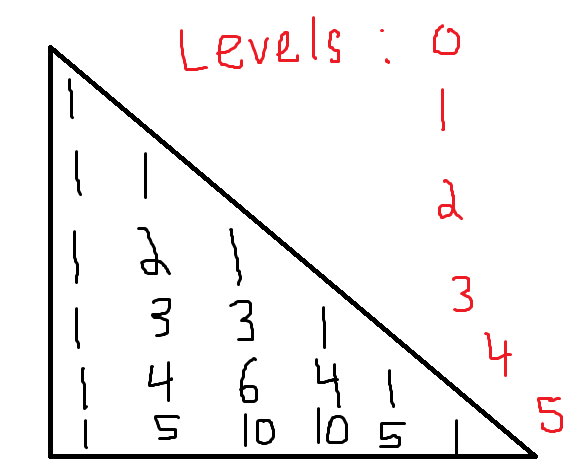
\includegraphics[scale = 1]{1.5.15-triangle.png}
	\end{center}
	
For a tree with $k=2^n$ nodes, there are $n+1$ levels.\\
Notice that the sum of each level corresponds to $2^n$ where n represents the level. For example; $n=0$ has a sum of 1, $n=4$ has sum of $16$ since $2^4$. $n=5$ has sum of $32$ since $2^5$. This is single depth.\\

By summing all levels until $n=4$, we get $32$ as total node depth. Recall single level nodes of $n=4$ was 16 node depth.\\

Therefore, $Avg \thickspace node \thickspace depth$: $\frac{single \thickspace node \thickspace depth}{total \thickspace node \thickspace depth}$.

For example; $\frac{16}{32}$ results in $\frac{1}{2}$.\\

So total node depth increases by 2 each time.\\

We can also prove this by induction. $Avg \thickspace node \thickspace depth$: $\frac{n+1}{2}$

\end{document}
